
\documentclass{article}
\usepackage{fullpage}
\usepackage{graphicx}
\usepackage{listings}
\usepackage{tabularx}
\begin{document}
\section{Part A: Tracking Process Activity}

\subsection{Hardware Information}

\begin{center}
\begin{tabular}{|l|l|}
  	\hline
  	CPU name & Intel Core i7-3610QM CPU \\ \hline
  	CPU speed & 2.30GHz \\ \hline
  	L1 Cache Size & 32 KB \\ \hline
	L2 Cache Size & 256 KB \\ \hline
	L2 Cache Size & 6144 KB \\ \hline
	Memory & 5995 MB \\ \hline
\end{tabular}
\end{center}

\subsection{Initialization}

This experiment was done on my personal computer, that is running Linux Ubuntu 14.04 LTS OS. ALso CPU affinity was set to CPU 0 in order to get accurate readings

\subsection{Experimenting with CPU Frequency}

In order to measure CPU frequency I caculated multiple sleep calls in a loop so that the ith sleep waits $i/2$ seconds and during that time the number of cycles is measured. Once I got multiple frequency measurements I sorted them using quicksort and then tried to find the pair of CPUs that were the closest\/clustered and took the highest measurement of the pair. 

I ended up getting a CPU Frequency of 2294 MHz, which is pretty close to 2.3 GHz.

\subsection{Experiementing with Threshold}

I determined threshold through running the experimentation multiple times, first starting at 1000 and increasing the value by 500 until consistent results were produced. I ended up  staying with a threshold of 2500.

\subsection{Conclusion}

Results for this experiment were placed in a file called part\_a\_output.txt, and was called using run\_experiment\_A 30.

Some measurements below: \\

total inactive time,  0.189322 ms \\ 

total time, 84.064094 ms \\
active time, 83.874772 ms \\
average active time, 2.89223 ms \\


By observation, since we have a CPU Frequency of 2.3GHz and average active time of 2.89223 ms than we can say an interrupt occurs about every 6,652,129 cycles from (2.89223 * 1000 * 2300). There are also periods that have short durations, such as less than 1 ms, which suggests it is a little inconsistant with regular timer intervals which I suggest are the ones that happen after every 3 to 4 ms activity. These early interrupts could have been due to processes running in the back such as Google Chrome or Text Editor Sublime.
The total time of the experiment was 84.064094 ms and total interrupt time is 0.189322 ms, Therefore the percentage of time lost due to interrupts was 0.023\% of the total time.

\begin{figure}
\centering
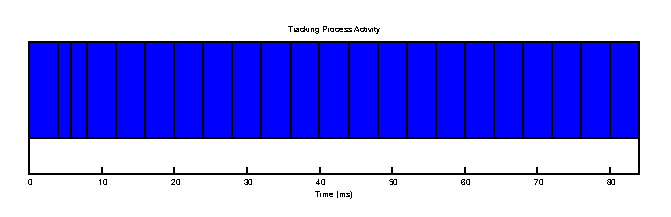
\includegraphics[scale=1.25]{part_a.eps}
\caption{Active \- Interval(BLUE) Inactive \- Interval(RED)}
\label{fig:parta}
\end{figure}

\section{Part A2: Measuring Context Switch Time}

\subsection{HARDWARE INFO AND SETUP}

In this section we measure the context switch time. When two share a CPU, the operating system schedules the processes which results in the CPU switching contexts between the different processes. Our approach was to measure the time between two on a single CPU. To do this, I forked off processes which measure their own active/inactive intervals, and find the duration where one child process is scheduled off the CPU and another child process takes over. 

\subsection{METHOD}

In the benchmark program part\_a2, I start the counter in the parent process, then spawn off a number of child process which begins measuring their own active/inactive periods in the same way as partA1. The intervals collected is processed in scripts/run\_experiment\_A2 to extract the context switch periods as well as plot the activity of each processes in part\_a2.eps. 

 
\subsection{CONCLUSION}
As you can see from graphs \ref{fig:parta2}, the length of time each process gets to run before it is forced to switch to another process varies based upon the number of process contending for the CPU. With two child processes there seems to be about 10 context switches within as span of 20 ms each active process lasting almost 3 ms each, however Child 0 seems to be prioritized at certain intervals. I believe this version of Linux is also running a CFS (Completely Fair Scheduler) however it doesn't seem to give each process a fair share of reasources after an interval of about 20 ms, this could be due to the specific Ubuntu OS.

Based on the output of run\_experiment\_A2, the average context switch time is 2.537 ms, this was due to the irregular periods when child 0 was prioritized for certain consistent periods which was explained above.

\begin{figure}
\centering
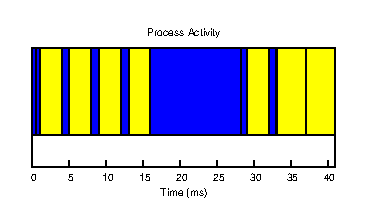
\includegraphics[scale=1.25]{part_a2.eps}
\caption{Process activity with two child processes}
\label{fig:parta2}
\end{figure}


\section{Part B: Measuring Numa Effects}
\subsection{Hardware Information}

This experiement was done on the wolf server.

\begin{center}
\begin{tabular}{|l|l|}
  	\hline
  	CPU name & AMD Opteron Processor 6348\\ \hline
  	CPU speed & 2.80GHz \\ \hline
  	L1 Cache Size & 64 KB \\ \hline
	L2 Cache Size & 2048 KB \\ \hline
	L3 Cache Size & 6144 KB \\ \hline
	Memory & 64408 MB \\ \hline
\end{tabular}
\end{center}

\subsection{Initialization}

Using the \"numactl --hardware\" command, I found that the machine (wolf.cdf) contains 4 nodes 

These nodes have about 12 CPU cores each, represented by the data collected below:

\begin{center}
\begin{tabular}{|l|l|}
  \hline
  Node & CPU \\ \hline
  0 & 0, 1, 2, 3, 4, 5, 6, 7, 8, 9, 10, 11 \\ \hline
  2 & 12, 13, 14, 15, 16, 17, 18, 19, 20, 21, 22, 23 \\ \hline
  4 & 24, 25, 26, 27, 28, 29, 30 ,31, 32, 33, 34, 35 \\ \hline
  6 & 36, 37, 38, 39, 40, 41, 42, 43, 44, 45, 46, 47 \\ \hline
\end{tabular}
\end{center}

With Node distances:

\begin{center}
\begin{tabular}{|l|l|l|l|l|}
	\hline
	Node Distances \\ \hline
	Node & 0 & 2 & 4 & 6 \\ \hline
  	0 & 10 & 16 & 16 & 16 \\ \hline
  	2 & 16 & 10 & 16 & 16 \\ \hline
  	4 & 16 & 16 & 10 & 16 \\ \hline
  	6 & 16 & 16 & 16 & 10 \\ \hline

\end{tabular}
\end{center}



\subsection{Test Script}

The results of our script can be found in part\_b\_output.txt and the script itself is run\_experiment\_B

\subsection{Observations}

From my results file mentioned above by looking at some of the operations from the CPUs below:

\begin{center}
\begin{tabular}{|l|l|l|l|l|}
	\hline 
	CPU & Copy & Scale & Add & Triad \\ \hline
	0 & 5842.4 & 5819.0 & 6559.7 & 6540.0 \\ \hline
	2 & 5853.9 & 5785.0 & 6429.5 & 6538.6 \\ \hline
	14 & 2970.5 & 2970.8 & 3014.5 & 3014.3 \\ \hline
	15 & 2974.2 & 2971.6 & 3017.1 & 3017.2 \\ \hline
	25 & 3694.6 & 3696.8 & 3939.3 & 3946.5 \\ \hline
	26 & 3687.4 & 3692.0 & 3933.4 & 3951.6 \\ \hline
	37 & 4004.9 & 4011.4 & 4228.2 & 4235.7 \\ \hline
	38 & 3909.0 & 3944.8 & 4136.8 & 4158.8 \\ \hline

\end{tabular}
\end{center}

The results show that CPU 0 and 2 are the ones with the highest bandwith.
This is expected since memory was binded specifically to node 0, and access to local memory will always be faster then remote access.
Also based on the table above it seems to be slightly inconsistant with the node distances shown above since CPUs 14 and 15 seem to have the lowest bandwidth, compared to the other 4 CPUs (25, 26, 37, 38) which have relativly closer bandwidth values.

\section{Appendix: Benchmark Tool Usage}
\subsection{run\_experiment\_A}
\begin{lstlisting}
Usage: run_experiment_A <n_intervals>
n_intervals = number of inactive periods for each process to record. Must be >= 0 
\end{lstlisting}
\subsection{run\_experiment\_A2}
\begin{lstlisting}
Usage: run_experiment_A2 <n_intervals>
n_intervals = number of inactive periods for each process to record.
\end{lstlisting}
\subsection{run\_experiment\_B}
\begin{lstlisting}
Usage: run_experiment_B
Outputs the result of running STREAM benchmark while binding memory on NODE 0, and
varying the CPUs in a list of (0,2,14,15,25,26,37,38).
\end{lstlisting}


\end{document}
